% !TEX encoding = UTF-8
% !TEX TS-program = pdflatex
% !TEX root = ../tesi.tex

%**************************************************************
\chapter{Framework Flutter e linguaggio Dart}
\label{cap:Framework Flutter e linguaggio Dart}
%**************************************************************

\intro{In questo capitolo viene inizialmente introdotto come un'applicazione mobile può essere sviluppata per poi concentrarsi su Flutter e tutte le sue componenti. Infine saranno mostrate come esempio alcune piccole applicazioni realizzate per imparare a utilizzare il framework Flutter.}\\

%**************************************************************
\section{Sviluppo applicazioni mobile}
Nel quotidiano, non solo in Italia ma in tutto il mondo, l'uso dello smartphone è in costante aumento.
Mentre fino a qualche anno fa il cellulare veniva usato solo per telefonare o mandare qualche messaggio, oggi lo smartphone viene utilizzato in qualsiasi ambito: lavoro, comunicare, divertirsi, video, musica o svago.
Ormai nei cellulari sono presenti applicazioni per qualsiasi esigenza ed è proprio per questo che chi sviluppa applicazioni ha dovuto considerare lo sviluppo per mobile come fattore primario.\\
	\begin{figure}[htbp]	
	\centering
	
\includegraphics[width=10cm]{immagini/sviluppoapp.png}
	\caption{Sviluppo applicazioni mobile}
	\label{fig:Sviluppo applicazioni mobile}
\end{figure}
\\
Esistono quattro diversi approcci di implementazione:
\begin{itemize}
	\item App native; 
	\item Web app; 
	\item App Ibride Web View Wrapper; 
	\item App Ibride Compile to Native.
\end{itemize}

\subsection{App native}
Il metodo nativo da la possibilità all'applicazione di integrarsi con la parte hardware del dispositivo, sfruttando così tutte le funzionalità del sistema operativo.
Le app native vengono realizzate utilizzando gli strumenti di sviluppo software e la documentazione fornita dai produttori del sistema operativo per il quale si ha l'intenzione di sviluppare.
Questo metodo è scelto sopratutto degli sviluppatori attenti alle prestazioni e alle performance dell'applicazione.
I vantaggi principali di sviluppare App native sono:
\begin{itemize}
	\item Maggiore velocità, affidabilità e reattività;
	\item Accesso diretto alla parte hardware e al software installato nel device; 
	\item Notifiche dirette;
	\item Funzionamento offline.
\end{itemize}
Attualmente i sistemi operativi più utilizzati sono:
\begin{itemize}
	\item Android; 
	\item iOS; 
	\item Windows Phone.\\
\end{itemize}


\subsubsection{Android}
\begin{figure}[htbp]	
	\centering
	
\includegraphics[width=1cm]{immagini/logoandroid.png}
	\caption{Logo Android}
	\label{fig:Logo Android}
\end{figure}
 Android è il sistema operativo più utilizzato e diffuso. È stato sviluppato da Google ed è stato scelto da multinazionali importanti come Samsung, Huawei e Amazon per il funzionamento dei loro dispositivi.
 Il linguaggio per sviluppare un'applicazione Android è Java. Negli ultimi anni è nato anche Kotlin che è un altro linguaggio ufficiale per la progettazione di applicazioni Android che è più moderno, meno complesso ma performante e compatibile con l'ambiente Android quanto Java.
 \newpage

 \subsubsection{iOS}
 \begin{figure}[htbp]	
 	\centering
 	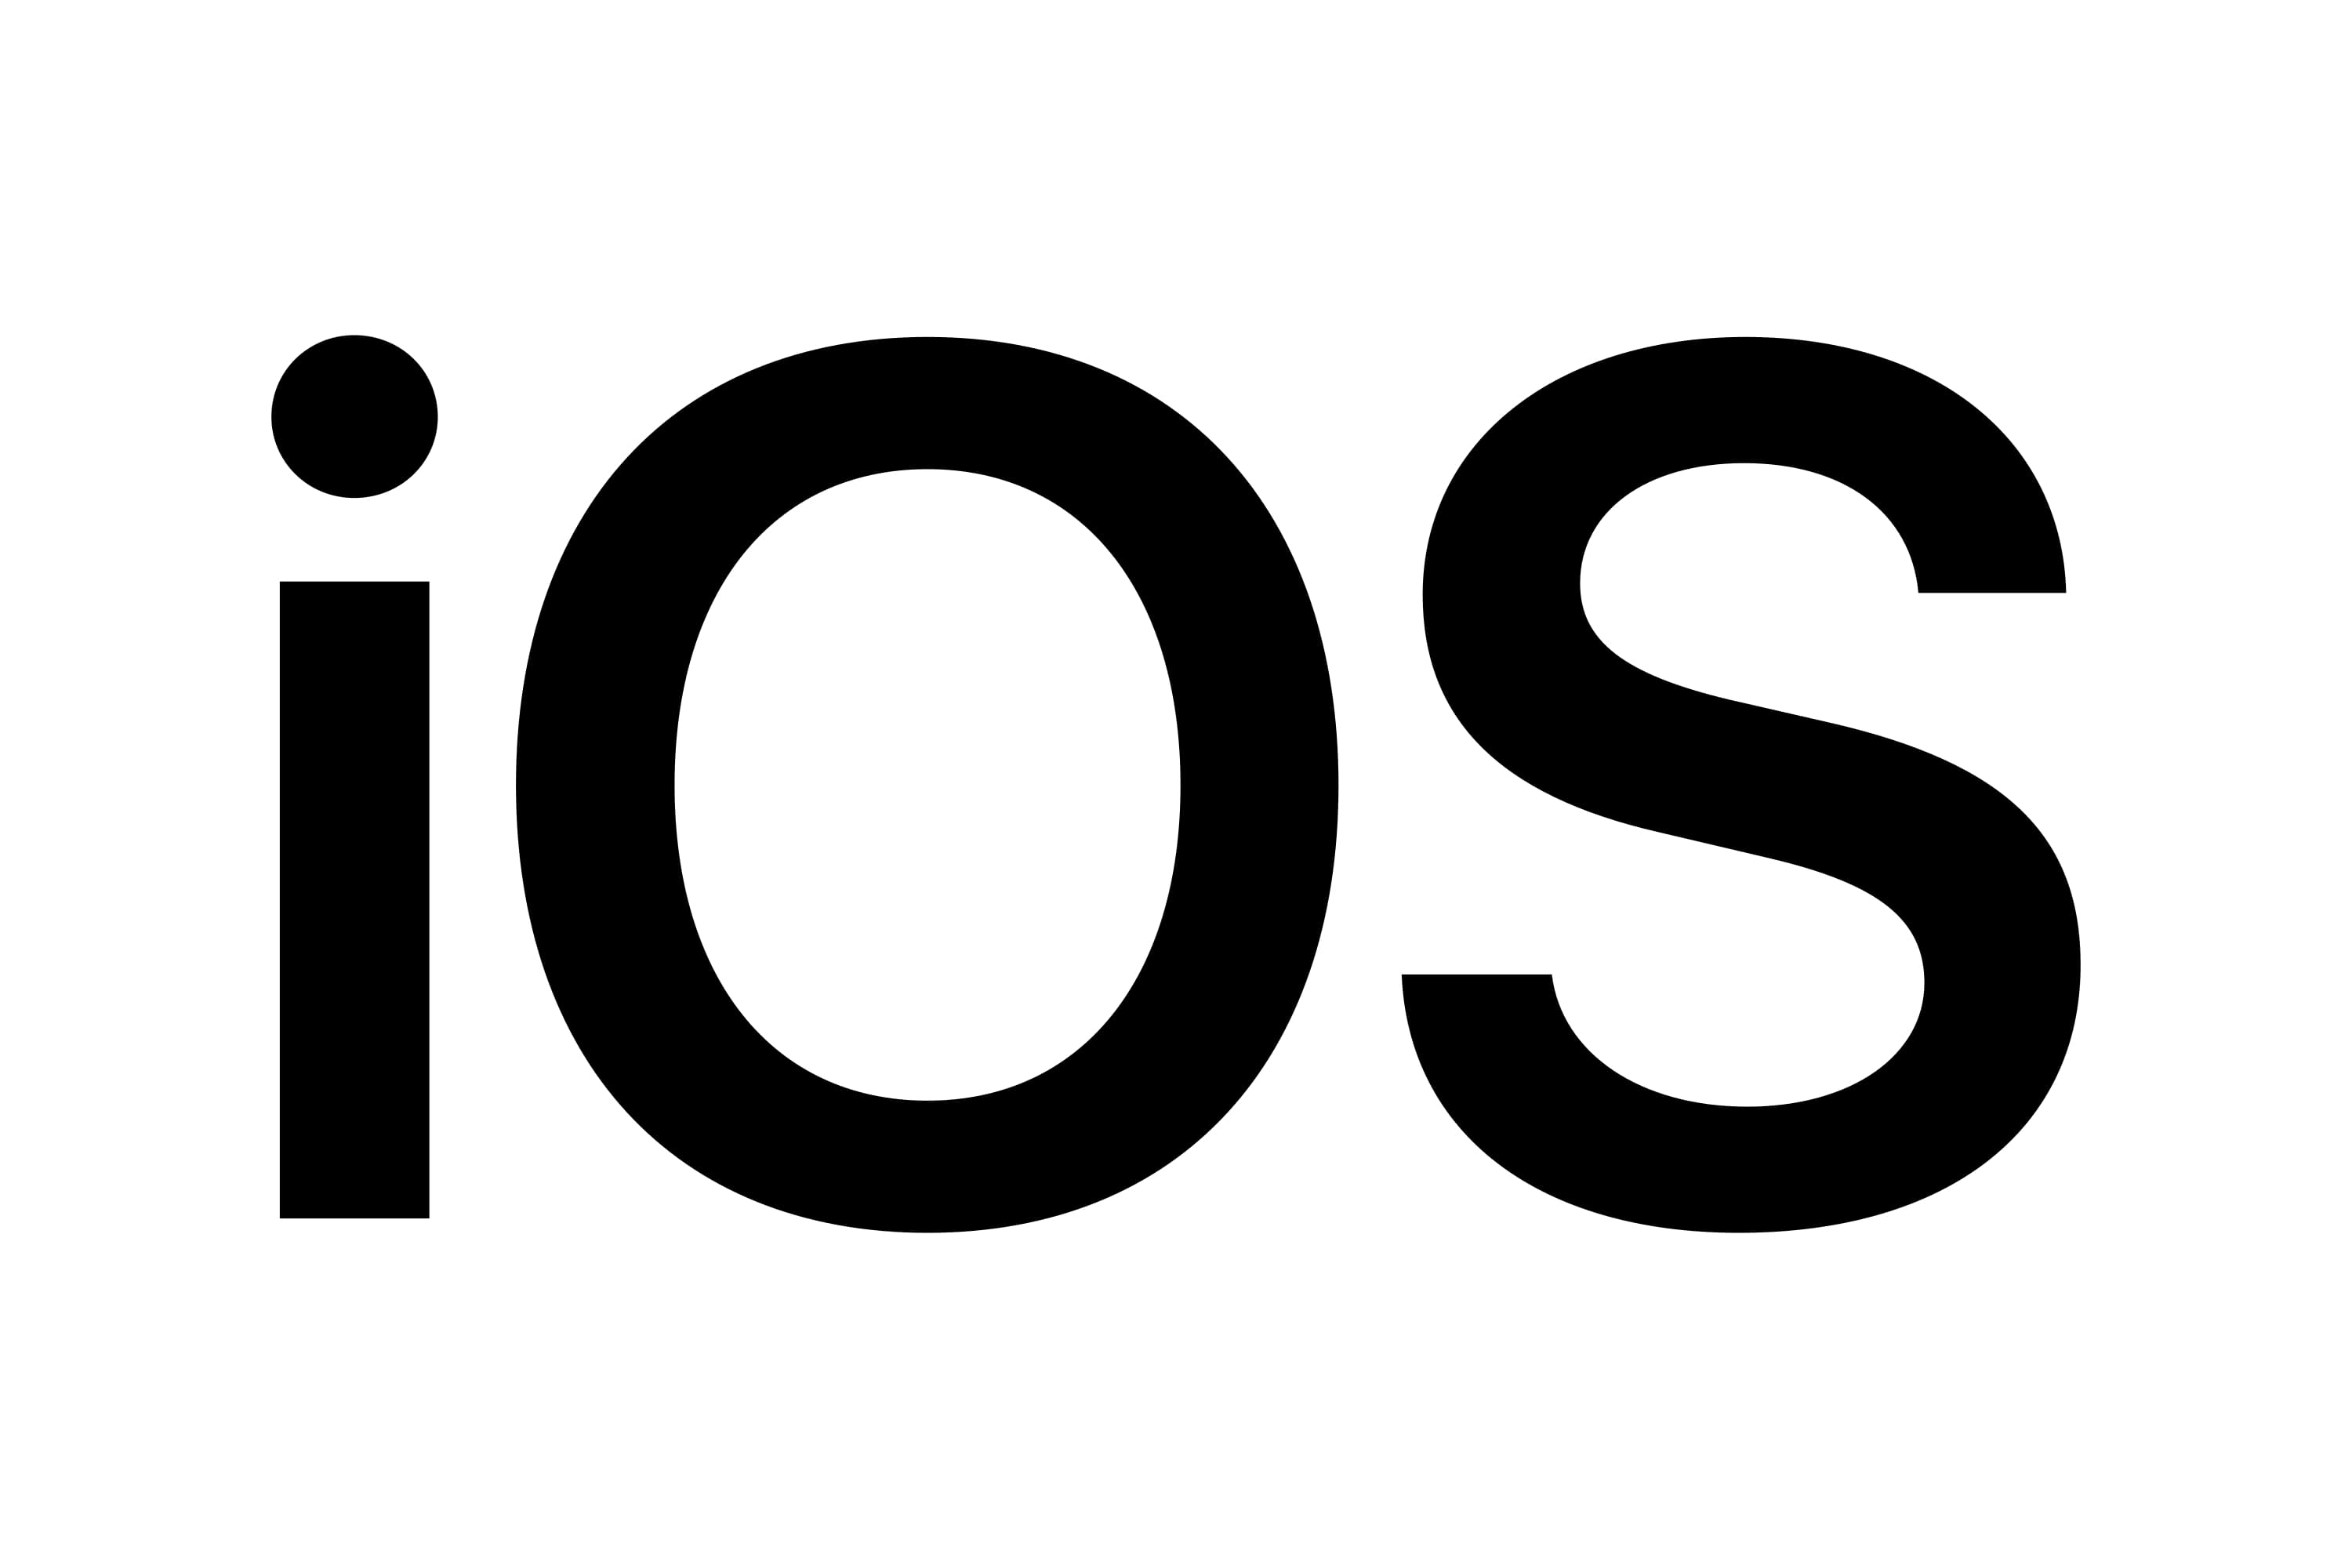
\includegraphics[width=1cm]{immagini/logoios.jpg}
 	\caption{Logo iOS}
 	\label{fig:Logo iOS}
 \end{figure}
 iOS è il sistema operativo sviluppato da Apple per dispositivi iPhone, iPod touch e iPad.
 Per un lungo periodo il linguaggio per sviluppare un'applicazione iOS è stato Objective-C che deriva da C e C++. 
 Per aumentare la produttività Apple ha lanciato un linguaggio di più alto livello ovvero Swift. Swift è veloce, più leggibile e meno prolisso. Nonostante ciò, Objective-C viene ancora preferito quando si sta lavorando più a basso livello.

 \subsubsection{Windows Phone}
 \begin{figure}[htbp]	
 	\centering
 	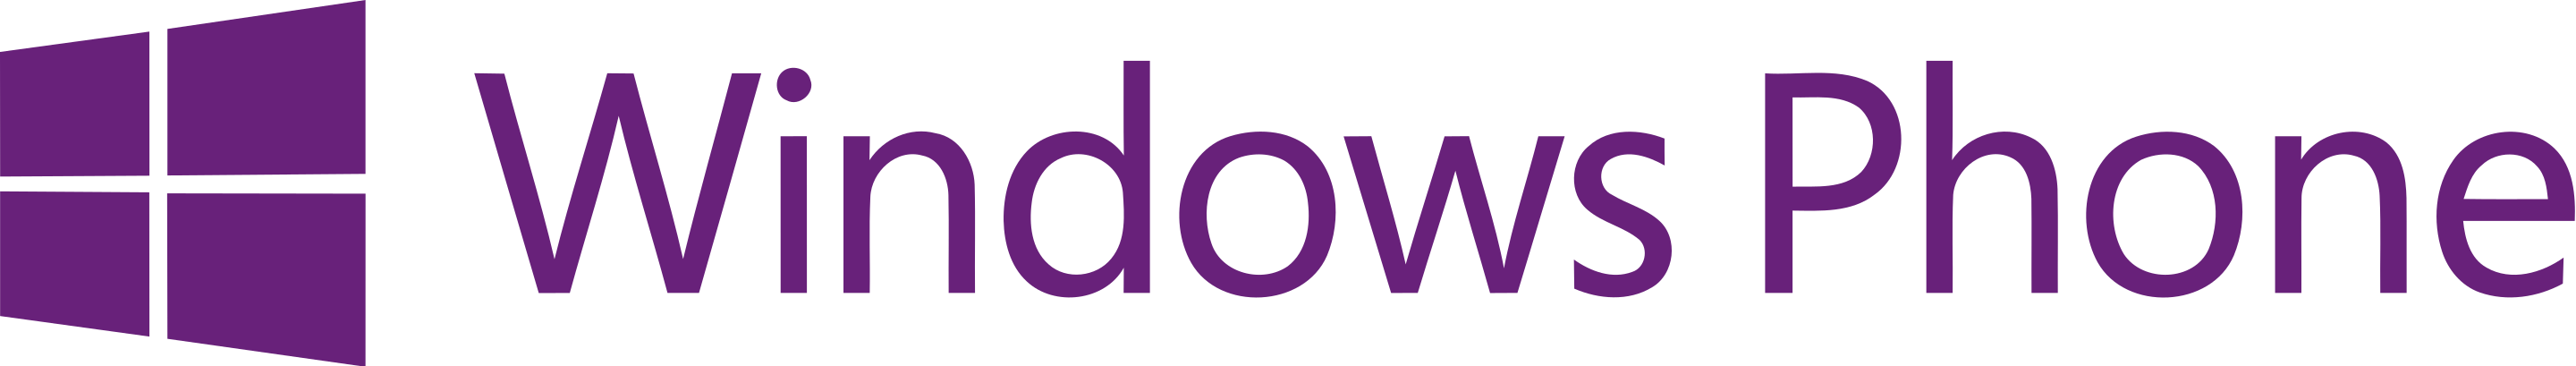
\includegraphics[width=3cm]{immagini/logowindowsphone.png}
 	\caption{Logo Windows Phone}
 	\label{fig:Logo Windows Phone}
 \end{figure}
Windows Phone è il sistema operativo sviluppato da Microsoft.
Il linguaggio utilizzato per sviluppare un'applicazione Windows Phone è C\# che è un linguaggio semi-compilato orientato agli oggetti.
Con Android e iOS in ambito mobile non c'è paragone. Invece per quanto riguarda sistemi desktop Windows risulta una delle migliori.\\
 
\subsection{Web app}
Una web app è un'applicazione che funziona come un sito web adattandosi al dispositivo utilizzato.
Queste applicazioni non necessitano di essere installate sugli smartphone e quindi non andranno ad aumentare la memoria utilizzata nel dispositivo. Inoltre non possono essere nemmeno pubblicate sugli Store e quindi non godono di questa enorme visibilità.
I principali framework e librerie per creare una web app sono:
\begin{itemize}
	\item Angular; 
	\item PolymerJS; 
	\item React.
\end{itemize}
I vantaggi di sviluppare una web app sono:
\begin{itemize}
	\item Scritte con Markup HTML;
	\item non essendo pubblicate sul Market non devono essere sottoposte al processo di approvazione; 
	\item Minor tempo di sviluppo.
\end{itemize}
\newpage
\subsection{App Ibride Web View Wrapper}
Questo tipo di metodo permette di creare applicazioni senza alcuna conversione del codice in base al sistema operativo. In pratica l'applicazione rileva inizialmente il sistema operativo utilizzato e successivamente imita l'aspetto dell'interfaccia utente utilizzando CSS, Sass...\\
Le piattaforme più usate sono:
\begin{itemize}
\item Ionic; 
\item Apache Cordova; 
\item PhoneGap.
\end{itemize}
I vantaggi principali di Ionic e delle App Ibride Web View Wrapper sono:
\begin{itemize}
	\item Riutilizzo facile del codice; 
	\item Ionic utilizza JavaScript e fornisce un supporto per Angular;
	\item Addatamento automatico in base alla piattaforma; 
\end{itemize}
Lo svantaggio principale di questo tipo di applicazioni sta in termini di velocità di calcolo e quindi avranno prestazioni inferiori a quelle compilate in nativo.

\subsection{App Ibride Compile to Native}
Le applicazioni ibride che compilano in nativo utilizzano un unico linguaggio di programmazione per la scrittura del codice. Una volta compilato i componenti dell'interfaccia utente del codice vengono convertiti nei componenti dell'interfaccia utente nativi.
Ad esempio se bisogna creare un nuovo Widget questo una volta compilato verrà tradotto nel Widget nativo del sistema operativo di esecuzione.
Le principali piattaforme utilizzate per compilare in nativo sono:
\begin{itemize}
	\item React Native; 
	\item NativeScript; 
	\item Xamarin; 
	\item Flutter.
\end{itemize}
I vantaggi principali di utilizzare piattaforme che compilano in nativo sono:
\begin{itemize}
	\item Anche se minore delle App Ibride Web View Wrapper hanno un elevata riutilizzabilità del codice; 
	\item Elevato numero di librerie utilizzabili;  
	\item Compilando in nativo offrono prestazioni elevate.
\end{itemize}
\newpage
\section{Flutter}
\begin{figure}[htbp]	
	\centering
	
\includegraphics[width=5cm]{immagini/flutterlogo.jpg}
	\caption{Logo Flutter}
	\label{fig:Logo Flutter}
\end{figure}

\subsection{Dart}

\subsection{Componenti}

\subsubsection{Framework}

\subsubsection{Engine}
Skia
\subsubsection{Embedder}

\subsection{Widget}

\subsubsection{Stateless widget}

\subsubsection{Stateful widget}

\subsubsection{Librerie Material e Cupertino}

\subsubsection{Principali Widget}

\subsection{Rendering e Layout}

\subsection{Esempi piccole applicazioni realizzate}
